\documentclass[
    11pt,
    spanish,
    a4paper
]{article}
%\usepackage[a4paper,left=.4in,right=.4in,top=1in,bottom=1in]{geometry}
\usepackage[utf8]{inputenc}
\usepackage[spanish]{babel}
\usepackage{authoraftertitle}
\usepackage{booktabs}
\usepackage{breqn}
\usepackage{caption}
\usepackage{float}
\usepackage{graphicx}
\usepackage{listings}
\usepackage{verbatim}

\def\doctype{Trabajo práctico}
\title{Ejercicios de FT \& RDB}
\author{Gonzalo Nahuel Vaca}

\begin{document}

\makeatletter
\begin{titlepage}
	\begin{center}
		\vspace*{1cm}

		\Huge
		\textbf{\doctype}
		\vspace{0.5cm}

		\LARGE
		\@title
		\vspace{0.5cm}

		\textbf{Introducción a los sistemas críticos}

		\vspace{1.5cm}

		\textbf{\@author}

		\vspace{1.5cm}

		
\includegraphics[width=0.8\textwidth]{img/logoFIUBA.pdf}

		\vfill
		Maestría en Sistemas Embebidos\\
		Universidad de Buenos Aires\\
		Argentina\\
		\today
	\end{center}
\end{titlepage}
\makeatother
\newpage

\section{Ejercicio 1}

En la figura \ref{fig:rdboriginal} se observa el RDB del ejercicio.

\begin{figure}[htbp]
	\centering
	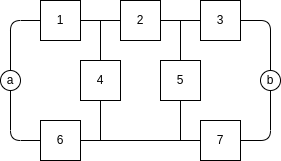
\includegraphics[width=0.5\textwidth]{img/rdb.png}
	\caption{RDB del ejercicio.}
	\label{fig:rdboriginal}
\end{figure}

A partir de la figura \ref{fig:rdboriginal} se identificaron los caminos posibles:

$$ c_1 = (x_1 \cap x_2 \cap x_3) $$
$$ c_2 = (x_6 \cap x_7) $$
$$ c_3 = (x_1 \cap x_4 \cap x_7) $$
$$ c_4 = (x_1 \cap x_4 \cap x_5 \cap x_3) $$
$$ c_5 = (x_6 \cap x_4 \cap x_2 \cap x_3) $$
$$ c_6 = (x_6 \cap x_4 \cap x_2 \cap x_5 \cap x_7) $$

Finalmente el RDB paralelo queda de la siguiente manera:

\begin{figure}[htbp]
	\centering
	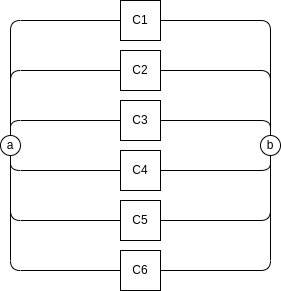
\includegraphics[width=0.5\textwidth]{img/rdb_paralelo.png}
	\caption{RDB paralelo.}
	\label{fig:rdbparalelo}
\end{figure}

\begin{dmath}
	\theta = (x_1 \cap x_2 \cap x_3) \cup (x_6 \cap x_7) \cup (x_1 \cap x_4 \cap x_7) \cup (x_1 \cap x_4 \cap x_5 \cap x_3) \cup (x_6 \cap x_4 \cap x_2 \cap x_3) \cup (x_6 \cap x_4 \cap x_2 \cap x_5 \cap x_7)
\end{dmath}

\section{Ejercicio 2}

En la figura \ref{fig:rdbequivalente} se puede observar un modelo RDB equivalente.

\begin{figure}[htbp]
	\centering
	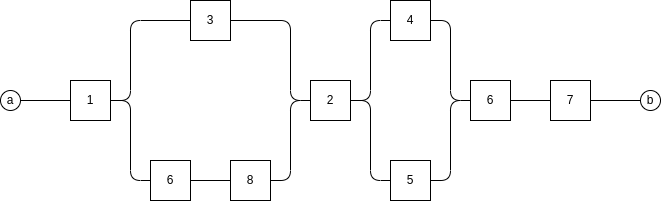
\includegraphics[width=\textwidth]{img/rdb2.png}
	\caption{RDB del equivalente.}
	\label{fig:rdbequivalente}
\end{figure}

A continuación se observa su función de estructura:

\begin{dmath}
	\theta = x_1 \cap (x_3 \cup (x_6 \cap x_8) ) \cap x_2 \cap (x_4 \cup x_5) \cap x_6 \cap x_7
\end{dmath}

\newpage

\section{Ejercicio 3}

En la figura \ref{fig:rdbcreado} se puede observar el RDB del circuito.

\begin{figure}[htbp]
	\centering
	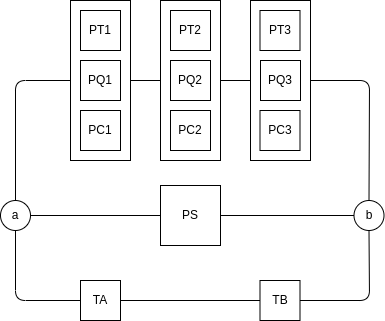
\includegraphics[width=0.5\textwidth]{img/rdb3.png}
	\caption{RDB del circuito.}
	\label{fig:rdbcreado}
\end{figure}

$$ \theta = ((PT_1 \cup PQ_1 \cup PC_1) \cap (PT_2 \cup PQ_2 \cup PC_2) \cap (PT_3 \cup PQ_3 \cup PC_3)) \cup PS \cup (T_a \cap T_b) $$

En la figura \ref{fig:arbol} se puede observar el árbol de fallas.

\begin{figure}[htbp]
	\centering
	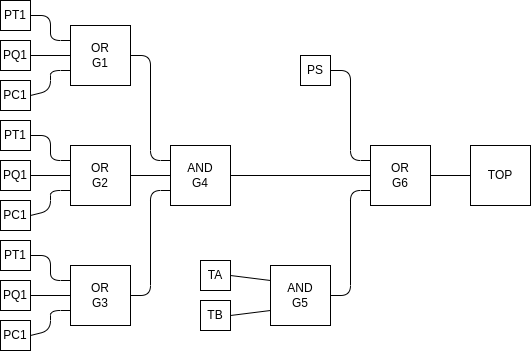
\includegraphics[width=0.8\textwidth]{img/arbol.png}
	\caption{Árbol de falla.}
	\label{fig:arbol}
\end{figure}

Una mejora frente a los disparos espurios del sensor de presión sería poner una redundancia con lógica \emph{AND}.

\end{document}